\section{本土主義和中港矛盾為何在近年急速冒起?}

本土主義和中港矛盾近年來急速冒起,但「本土主義」所包含的範圍甚廣,不易說清。即使把討論限於相對排拒中國大陸的群體,仍有相當多不同甚至互相矛盾的立場。以移民政策為例,削減單程證數目、收緊申請單程證資格、修改《基本法》的居留權條文,以至剝奪已經取得居留權人士的身分,就是四種差距甚遠的倡議而後果各異。而正如其他的政治立場一樣,本土主義支持者的立場也可以相當流動,一時的說法往往不足作準。不過,總的來說,本土主義的支持者往往會認為香港社會對香港自主受威脅的警覺性不足,認為要加強保護香港社會、文化、政治和經濟等各方面,免受外界特別是中國大陸的控制。

從二零一一年開始,中港關係出現了兩個明顯轉向。首先,各式各樣從日常生活衝突引起的中港矛盾在社會爆發。承接而來的,是部分香港人對中國大陸所有事物採取全面抗拒的態度,無論任何和中國大陸相關的消息均作負面理解。儘管香港身分認同過去一直都以與中國認同作對照來建立,但會保持一定的情感紐帶,例如把反對中共管治和欣賞文化傳承區分開,也有所謂的「愛國不等於愛黨」;然而新一輪的中港矛盾卻不單止針對中共管治,更往往把一般中國大陸的平民百姓也連帶一起敵視。由於這改變涉及大量情感指控,背後的客觀環境因素往往不易說清。

首個通過日常生活突顯的中港矛盾,來自「雙非政策」所延伸出來的一系列問題。按《基本法》規定,在香港出生而父母其中一方是中國公民的嬰兒,不論父母是否香港永久性居民,一律自動成為香港永久性居民。而「雙非」的意思,就是父母雙方都不是香港永久性居民的嬰兒。自從香港開放個人遊,不少大陸居民以生育旅遊的方式來港產子,有些是為了逃避計劃生育,有些則希望為孩子取得香港戶籍和領取特區護照的資格。「雙非」嬰兒的數目,從二零零一年的620名,大幅增加二零一一年的32,653名,佔當時所有香港新生嬰兒的37\%。

\begin{figure}[htbp]
    \centering
    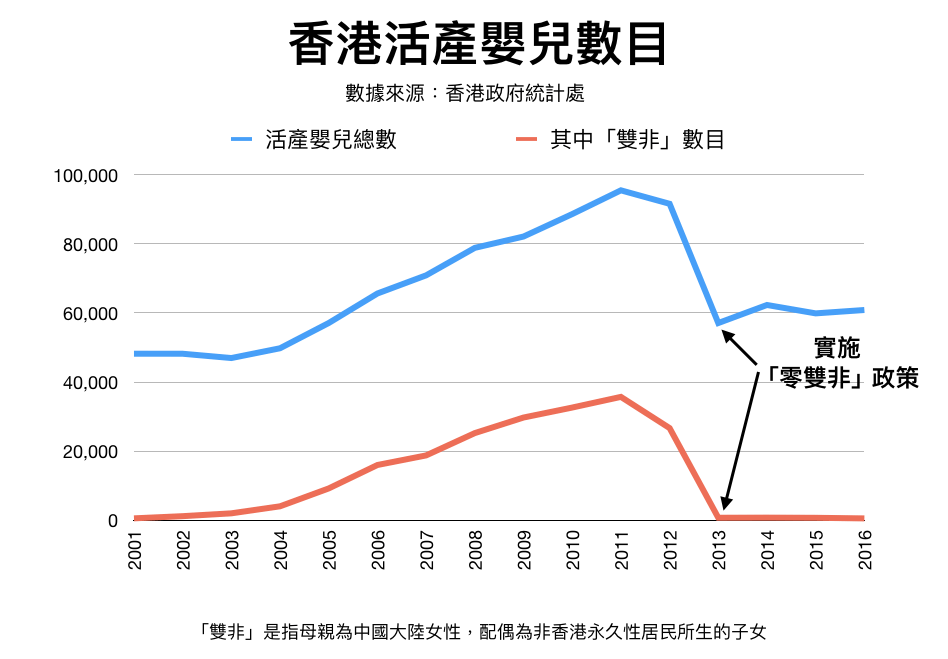
\includegraphics[width=0.7\textwidth]{c10/h-klesson1-013.png}
    \caption{抗爭中的新界石崗菜園村} 
\end{figure}

本來「雙非」問題是可以控制的,只要政府要求醫院拒絕「雙非」孕婦的分娩預約,並在入境口岸拒絕沒有預約的孕婦入境,便可解決問題。事實上,香港在二零一三年起實施了上述政策,「雙非」嬰兒的數目大幅回落到本來每年數百名的水平。不過,在該政策實施之前,香港政府曾經對「雙非」的立場十分正面,甚至認為可以幫助解決香港人口老化的問題。這個看法受到輿論的強烈批評,畢竟「雙非」嬰兒日後不一定在香港定居,卻隨時可以來港獲得永久性居民的待遇,日後無論是教育或各類社會保障均無從規劃需求。當時的香港政府立場,就被認為出賣了本地人的利益。

相對來說,八九民運後香港人對失去自由和人權的憂慮,還是比較遙遠和抽象。但當「雙非」嬰兒潮來到的時候,各種大陸人和本地人之間的衝突卻變得即時和不能迴避。醫院因為規劃沒有預設分娩數字爆升,於是就出現本地人和大陸人爭奪醫院床位的問題;之後輪到學校因為規劃沒有預設學童數字爆升,又出現本地人和大陸人爭奪學位。而對於「雙非」兒童的家長,他們自己沒有香港的居留權,只好舉家在深圳居住然後讓孩子每天天還未亮便要趕過境上學,對家長和孩子來說同樣是折騰。一個沒經過深思熟慮的人口政策,為各方都帶來沉重的負擔。

面對社會各界的聲討,梁振英就任特首後隨即改變政策,實施「零雙非」。不過中港矛盾沒有因而停止,反而在其他的議題上越演越烈,當中以「自由行」議題最為嚴重。「自由行」的正式名稱是港澳個人遊,自二零零三年開始實施,容許中國大陸居民透過簡單的個人簽注前往香港。在此政策之下,大陸訪港旅客高速增長,由二零零二年的638萬人次大幅度增加至二零一三年的4,075萬,為市民生活帶來巨大改變,不少評論認為其社會成本已遠超過其益處。旅客和本地人之間的衝突,更把中港矛盾變成日常生活的一部分。

政策的原意,是要促進香港的旅遊業,進而振興香港經濟。然而當旅客越來越多的時候,香港社會發現個人遊帶來的利益和成本分配並不平均,利益往往由一少撮人把持,而成本則由社會整體分擔。例如大陸旅客來港購物,通常會集中於一些講求品質的商品,例如珠寶首飾和藥物。於是乎,珠寶店和藥店便成為暴利行業,可以付得起高昂的租金壟斷遊客區的商舖,同一品牌的珠寶店可以在旺角同時設有接近二十間的分店。調查顯示於二零零四至二零一三年間,香港的化妝品店增加了十五倍。相對來說,售賣日用品的商店因為無法負擔同樣的租金,便唯有紛紛撤出。

當商鋪單一化的趨勢來到一些本來不是旅遊區的地方,便會嚴重干擾市民的日常生活。例如沙田新城市廣場原為區內六十多萬居民最主要的購物中心,但由於位處連接邊境的鐵路線上,便成為大陸旅客的購物熱點,原有店鋪例如診所、書報攤等紛紛被迫遷走。對於很多沙田居民來說,能夠從個人遊中得益的是商場業主,而他們則失去了一個本來屬於社區、服務社區的消閒空間。另一案例則為位於新界西北部的屯門區和元朗區。這兩處由於遠離市區,居民以低下階層為主。然而隨著西部口岸開通,屯門和元朗的地理位置對於深圳居民來說變得相當便捷。有開發商特設接駁專車,從口岸接送遊客到旗下商場購物,好讓他們可以賺取更高租金。和沙田的居民一樣,屯門和元朗的居民同樣不習慣自己生活的地方忽然變成遊客熱點,即使在居住區附近也要和拉著行李箱的旅客爭路。

沙田、屯門和元朗的案例,突顯了新增的來港旅客其實已不能稱之為遊客,因為他們的主要目的並非旅遊觀光,而是滿足其日常購買需求。這個改變的起因,來自香港政府一度開放深圳居民可無限次數來港,於是不少深圳居民把來港購物變成一種職業,透過帶貨過關來協助深圳的進口商逃避關稅,也就是所謂的「水貨客」。調查顯示到了二零一七年,百分之五十八的大陸旅客屬即日往返,並非傳統意義下的遊客。有組織的「水貨客」會集中搶購某些大陸熱門的日用產品,例如個別品牌的嬰兒奶粉,以致這些產品經常在市面斷貨,使本地消費者感到受威脅。

\begin{figure}[htbp]
    \centering
    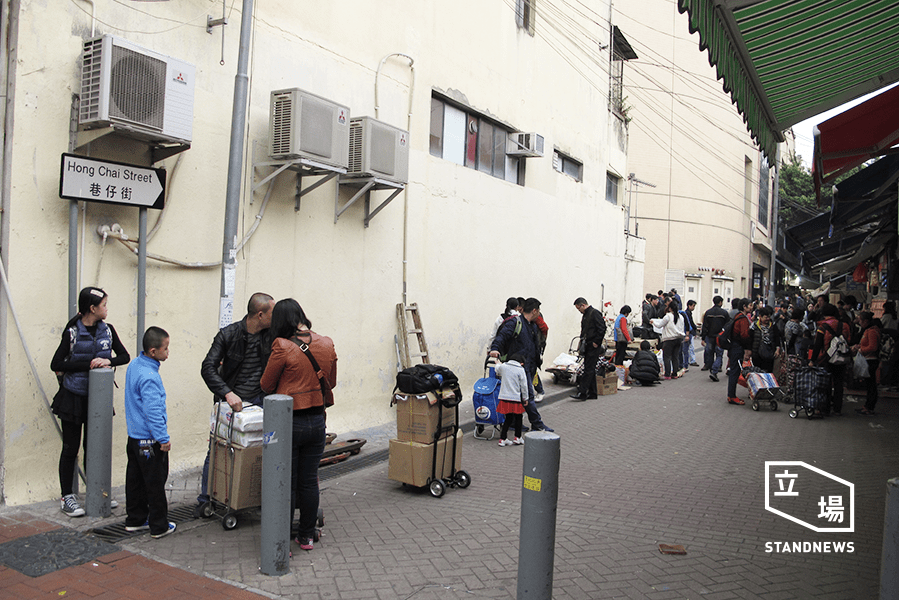
\includegraphics[width=0.7\textwidth]{c10/h-klesson1-014.png}
    \caption{北區一些街道變成「水貨客」的集散地} 
\end{figure}

更不幸的,是正如前文所述,中國政府近年刻意改變大陸傳媒有關香港的言論,向民眾灌輸錯誤觀念,也影響到一些大陸旅客在港的行為。當個別大陸旅客表達出「恩主心態」,即把市場交易視為一方向另一方的恩賜,而這些表現又被傳媒捕足廣傳,便很容易牽動很多香港人的反感。他們認為自己沒有享受到中港融合的好處,日常生活卻因大陸旅客的出現而大受影響,而這些旅客還要現出居高臨下的態度,情緒上便很容易把所有大陸人都視為在香港作亂的惡霸。

如是者,近年香港出現了一些針對大陸旅客的「光復行動」,不論對方是否真的是大陸旅客或「水貨客」,只要見到拉著行李箱和說普通話的便會圍著來辱罵甚至毀壞對方的行李箱。這些直接和激烈的回應方式,並非一時之間忽然出現,而是一個逐步走向激進的過程。示威者由要求鐵路職員嚴格執行運送行李數量的規定,發展至圍堵集中向大陸旅客售賣貨品的專門店,再變成直接針對大陸旅客。這些做法固然粗糙,台灣遊客之間就常流傳被誤認而受歧視的故事。肢體上的直接攻擊,更有違香港社會過去對和平理性抗爭的追求。換個角度來說,這些激烈抗爭正正代表了中港矛盾已在日常生活都中植根。

現實生活尚且如此,在網上世界則更為猖狂。在個別的網上群組和新聞媒體的留言欄中,對中國各方面的批評可以沒有底線。例如每當中國出現天災人禍,留言者必然歡呼雀躍,因為在他們的眼中「沒有一個中國人是無辜的」。如果有來自中國大陸的人在香港遇上任何麻煩,無論是交通意外或是被騙,均一律不值得任何同情,因為這些人都是「殖民者」,都是潛在的敵人。在不少人眼中,中港關係是一種戰爭關係,今天的香港在中國面前就和中日戰爭期間中國在日本面前一樣,是被強行剝奪了自身的價值和尊嚴。在這種邏輯下,對中國的任何人或事表示同情都是背叛香港。

這些說法無助化解僵局,很大程度上和大陸網上憤青罵「小日本」等的情緒發洩類似;不過若要解決問題,僅僅譴責仇恨言論並不足夠,也要追問這些中港矛盾從何而來,特別是中港政治關係的角色。舉個例,世界各地都出現過遊客過多的問題,當地政府都會想辦法應對。但在香港的特殊政治環境當中,卻會有不少游走中港之間的權貴會通過聲稱應該包容旅客過多帶來的任何問題,以表達對中國政府的忠誠。當客觀的社會問題被理解為政治上的敵我矛盾,尋求解決之道就變得更為困難,民間怨憤亦會變得更為激烈。


伸延閱讀:

陳智傑(2016):〈身分認同與建構他者:香港生活經驗中的中港關係〉,

張少強、 陳嘉銘、梁啟智編《香港社會文化系列》。

羅永生(2014):〈香港本土意識的前世今生〉,《思想》第26期。

網上資源:

\href{https://thestandnews.com/society/上水貨客-5-活在水貨店與藥房的夾縫中/}{立場報道(2015):〈活在水貨店與藥房的夾縫中〉:立場新聞,2015年2月6日}